
%(BEGIN_QUESTION)
% Copyright 2011, Tony R. Kuphaldt, released under the Creative Commons Attribution License (v 1.0)
% This means you may do almost anything with this work of mine, so long as you give me proper credit

One of the major processes used to treat municipal wastewater is {\it aeration}, where the dissolved oxygen concentration of the wastewater is enhanced by bubbling air through the water in an {\it aeration basin}.  A dissolved oxygen (``DO'') analyzer measures the oxygen concentration in the wastewater, and a controller varies the speeds of blowers pumping air into the basins using AC motors powered through variable-frequency drives (VFDs):

$$\includegraphics[width=15.5cm]{i04598x01.eps}$$

Suppose flow transmitter FT-19 fails with a high-flow signal.  Determine the effect this will have on the other two controllers in the system, and on the actual dissolved oxygen content of the wastewater over time.

\vfil 

\underbar{file i04598}
\eject
%(END_QUESTION)





%(BEGIN_ANSWER)

This is a graded question -- no answers or hints given!

%(END_ANSWER)





%(BEGIN_NOTES)

If FT-19 fails high, FIC-19 will cause the blower to shut off.  This in turn will cause the wastewater DO to fall, and the AIC will call for more air.  If the blower on controller FC-18 is powerful enough, the DO will come back up to setpoint, albeit slower than usual.  If the blower on controller FC-18 is not powerful enough to deliver air sufficient to aerate the wastewater, the DO will never return back up to setpoint.

\vskip 10pt

There is insufficient information given to determine whether or not one blower will be enough to maintain the dissolved oxygen concentration at setpoint.  However, if we knew the FIC output values prior to the failure of FT-19, we could make a good guess.  If FIC-18 happened to be outputting less than 50\% prior to the fault, there's a good chance it would have enough excess capacity to keep up with demand, running at roughly twice its former speed.

%INDEX% Control, strategies: cascade
%INDEX% Process: wastewater aeration (dissolved oxygen control)

%(END_NOTES)


